% Szablon pracy dyplomowej. W razie potrzeby można oczywiście dodawać nowe pakiety.
%DIF PREAMBLE EXTENSION ADDED BY LATEXDIFF
%DIF UNDERLINE PREAMBLE
\RequirePackage[normalem]{ulem}
\RequirePackage{color}\definecolor{RED}{rgb}{1,0,0}\definecolor{BLUE}{rgb}{0,0,1}
\providecommand{\DIFadd}[1]{{\protect\color{blue}\uwave{#1}}}
\providecommand{\DIFdel}[1]{{\protect\color{red}\sout{#1}}}
%DIF SAFE PREAMBLE
\providecommand{\DIFaddbegin}{}
\providecommand{\DIFaddend}{}
\providecommand{\DIFdelbegin}{}
\providecommand{\DIFdelend}{}
%DIF FLOATSAFE PREAMBLE
\providecommand{\DIFaddFL}[1]{\DIFadd{#1}}
\providecommand{\DIFdelFL}[1]{\DIFdel{#1}}
\providecommand{\DIFaddbeginFL}{}
\providecommand{\DIFaddendFL}{}
\providecommand{\DIFdelbeginFL}{}
\providecommand{\DIFdelendFL}{}
%DIF END PREAMBLE EXTENSION ADDED BY LATEXDIFF

\pdfoutput=1
\pdfcompresslevel=9
\pdfinfo
{
    /Author ()
    /Title ()
    /Subject ()
    /Keywords ()
}
\documentclass[a4paper,onecolumn,twoside,12pt]{mwrep}

\usepackage{algorithm}
\usepackage{tikz}
\usepackage{hhline}
\usepackage{fixltx2e}
\usepackage{caption}
\usetikzlibrary{arrows,shapes}

\usepackage{color}
\usepackage{algpseudocode}
\usepackage{times}
\usepackage[utf8x]{inputenc}
\usepackage[T1]{fontenc}
%\usepackage[polish]{babel}
\usepackage{polski}
\usepackage{setspace}
\usepackage{amsfonts}
\usepackage{amsmath}
\usepackage{array,longtable}
\usepackage{pdflscape}
\usepackage{afterpage}
\usepackage{backref}
\usepackage{array, makecell} %
\usepackage{tabularx}
    \newcolumntype{L}{>{\raggedright\arraybackslash}X}

\renewcommand*{\backref}[1]{}
\renewcommand*{\backrefalt}[4]{%
    \ifcase #1 (Brak cytowania.)%
    
    \or        (Cytowanie na stronie~#2.)%
    \else      (Cytowanie na stronach~#2.)%
    \fi}
\renewcommand*{\backreftwosep}{ i~}%
\renewcommand*{\backreflastsep}{ i~}%
\newcolumntype{L}{>{\raggedright\arraybackslash}X}

\hyphenpenalty=10000
\clubpenalty=10000	
\widowpenalty=10000	
\brokenpenalty=10000
\exhyphenpenalty=999999	
\righthyphenmin=3

\newcolumntype{C}{>{\rowfont}c}
\newcolumntype{C}{>{\rowfont}c}
\newcommand\setrowfont[1]{\noalign{\gdef\rowfont{#1}}}
\gdef\rowfont{}

\tolerance=4500
\pretolerance=250
\hfuzz=1.5pt
\hbadness=1450

\renewcommand{\labelitemi}{$\bullet$}

\makeatletter
\newcommand{\newalgname}[1]{%
  \renewcommand{\ALG@name}{#1}%
}
\newalgname{Algorytm}
\renewcommand{\listalgorithmname}{Liste des \ALG@name s}
\makeatother

\newcommand*\conj[1]{\bar{#1}}
\newcommand*\mean[1]{\bar{#1}}
\newcommand{\norm}[1]{\left\lVert#1\right\rVert}

\newcommand{\LongComment}[1]{\Comment{\parbox[t]{.45\linewidth} {#1}}}

\sloppy

\setlength{\textwidth}{\paperwidth}
\addtolength{\textwidth}{-5cm}
\setlength{\textheight}{\paperheight}
\addtolength{\textheight}{-5cm}
\setlength{\oddsidemargin}{0.0cm}
\setlength{\evensidemargin}{0.0cm}
\topmargin -1.25cm
\footskip 1.4cm

\linespread{1.5}

\begin{document}

\setcounter{page}{1}
\pagestyle{plain}
\tableofcontents

\chapter{Wstęp}\label{chap:introduction}

\section{Problematyka i zakres pracy}
Niniejsza praca dotyczy zakresu inżynierii oprogramowania, a w szczególności aplikacji przeznaczonej na urządzenia mobilne. Jej działanie jest dodatkowo wspierane przez webową aplikację serwerową, która ma dostęp do bazy danych.

W ostatnich latach nastąpił intensywny rozwój technologiczny telefonów komórkowych. Wzrost wydajności oraz umieszczanie w nich dodatkowych modułów sprawiły, że urządzenia mobilne zaczęły być wykorzystywane do celów innych niż komunikacja. Jednym z nich jest wspieranie różnego rodzaju aktywności sportowych, między innymi biegania. Aplikacje mogą wykorzystywać otrzymywane poprzez protokół bluetooth dane z mierników tętna lub aktualną lokalizację użytkownika pobieraną z wbudowanego w urządzenie modułu lokalizacji.

W momencie pisania niniejszej pracy na rynku znajduje się wiele takich aplikacji, a ich funkcjonalność opiera się głównie na analizie odbytych treningów. Użytkownik przeważnie ma możliwość wyświetlenia przebiegu pokonanej trasy na mapie, sprawdzenia ile czasu zajął bieg, jaki był całkowity przebyty dystans, a także porównania statystyk z poszczególnych fragmentów trasy. Niektóre z nich oferują także pewne funkcje społecznościowe. Możliwe jest zapisywanie przebiegu pokonanej trasy, a następnie udostępnienie jej. W wyniku tego działania inni biegacze mają możliwość wyszukania trasy i odbycia na niej treningu we własnym zakresie. W przypadku niektórych aplikacji użytkownicy mają dodatkowo możliwość porównania swojej próby na konkretnej trasie z próbami innych zawodników na podstawie całkowitego czasu treningu. Aplikacje zawierające wymienione powyższe funkcje mają jednak pewne braki i niedoskonałości.

Po pierwsze, zawody biegowe różnią się od siebie dystansem i rodzajem terenu - niektóre wiodą przez trasę o twardej nawierzchni (na przykład asfalt, kostka brukowa) i wyrównanym poziomie, zaś inne przez nieutwardzone grunty wymagające podbiegów i zbiegów. Choć na pierwszy rzut oka może nie wydawać się to oczywiste, przygotowanie do startu w konkretnych zawodach jest najefektywniejsze wtedy, gdy trening przeprowadzany jest w warunkach zbliżonych do tych, które można spotkać na trasie biegu. Z tego względu użytkownicy poszukujący trasy, zwykle mają co do niej pewne preferencje, które nie mogą zostać uwzględnione, ponieważ kryteria wyszukiwania tras w istniejących aplikacjach są bardzo ograniczone.

Po drugie, mimo że porównanie czasów osiągniętych na poszczególnych trasach jest dobrym sposobem na sprawdzenie swojej obecnej formy, istniejące aplikacje umożliwiają sprawdzenie rezultatu dopiero po zakończonym treningu, a nie w jego trakcie.

Z tych względów, głównym przedmiotem pracy jest zaprojektowanie i stworzenie aplikacji, której funkcjonalność jest udoskonalona i w efekcie nie posiada wymienionych problemów. Do każdej z tras udostępnianych przez społeczność zostaną przypisane pewne cechy. Ich określanie dokonywane będzie automatycznie, jednak biegacz tworzący trasę będzie miał możliwość skorygowania niedokładności we własnym zakresie. Są one następujące:
\begin{itemize}
\item całkowita długość wyrażona w kilometrach,
\item nachylenie terenu,
\item twardość nawierzchni wyrażona w procentach - określa jaka część całej trasy prowadzi przez grunt utwardzony.
\end{itemize}
Użytkownik ma możliwość określenia kryteriów wyszukiwania powiązanych z cechami trasy. Dodatkowo może on określić maksymalny promień wyszukiwania względem jego obecnej pozycji. W ten sposób otrzymuje on rezultat zawierający znajdujące się dostatecznie blisko trasy spełniające jego wymagania, przez co przygotowanie do zawodów może być efektywniejsze. Tempo biegacza może zmieniać się na różnych fragmentach trasy, a więc osoba zajmująca pierwszą pozycję w połowie zawodów, niekoniecznie je zwycięży. Mając to na uwadze możliwe jest udoskonalenie drugiego aspektu z aktualnie istniejących aplikacji. Na podstawie prób zawodników którzy ukończyli wcześniej konkretną trasę, użytkownik będzie informowany nie tylko o ostatecznie osiągniętej pozycji, lecz także o aktualnie zajmowanym miejscu w klasyfikacji na poszczególnych fragmentach trasy oraz o fakcie, że zyskał lub utracił pozycję. Taka symulacja sprawia wrażenie uczestnictwa w wirtualnych zawodach. Uczucie rywalizacji z innymi, może nie tylko urozmaicić trening, ale także sprawić, że za sprawą chęci wygranej, będzie on efektywniejszy.

\section{Cele pracy}
Do celów niniejszej pracy należą:
\begin{itemize}
\item \textbf{Opracowanie modelu danych pozwalającego na przechowywanie dodatkowych informacji o zapisywanych trasach wraz z rozwiązaniem problemu charakterystyki tras oraz wirtualnej rywalizacji} - pierwszym z działań które należy podjąć, jest zaprojektowanie modelu danych. Tworzone trasy muszą być zapisywane w sposób umożliwiający określanie ich cech (zarówno automatyczne jak i manualne na podstawie opinii użytkownika), wyszukiwanie na podstawie wprowadzonych kryteriów oraz przeprowadzanie procesu wirtualnej rywalizacji. Jako że aplikacja składa się z funkcjonalności, do których działania wymagana jest komunikacja pomiędzy użytkownikami, model danych musi zostać opracowany nie tylko dla aplikacji mobilnej, lecz także dla części serwerowej systemu. Następnie należy opracować logikę, która pozwoli przypisać trasie pewne cechy. Charakterystyka będzie jedynie sugestią, dlatego użytkownik powinien mieć możliwość ich skorygowania. Ostatnim elementem jest zaproponowanie podejścia, które na podstawie poprzednich prób użytkowników, pozwoli przeprowadzić swego rodzaju „wirtualny wyścig”.
\item \textbf{Stworzenie prototypu mobilnej aplikacji wspomagającej trening biegaczy} - Dotyczy implementacji założeń opracowanych w pierwszym celu oraz zbudowaniu systemu składającego się z aplikacji mobilnej przeznaczonej na system operacyjny Android i aplikacji serwerowej posiadającej dostęp do bazy danych. Całość powinna być zaprojektowana w sposób, który w przyszłości umożliwi ewentualną obsługę kolejnego mobilnego systemu operacyjnego bez modyfikacji istniejącego kodu źródłowego.
\item \textbf{Ocena możliwości praktycznych stworzonego prototypu poprzez porównanie do istniejących aplikacji o podobnym zastosowaniu} - Na końcu stworzony system zostanie porównany z innymi, znajdującymi się już na rynku, rozwiązaniami w dziedzinie aplikacji treningowych. Na tej podstawie możliwa będzie ocena, czy rzeczywiście oferuje on rozszerzoną funkcjonalność.
\end{itemize}

\section{Przegląd literatury}
Niniejszy podrozdział zawiera pozycje, na które warto zwrócić uwagę, w przypadku potrzeby zgłębienia tematu podejmowanego w ramach pracy.
\subsection{Wykorzystywanie nawigacji satelitarnej}
\subsection{Budowanie aplikacji mobilnych}
\subsection{Budowanie aplikacji serwerowych}
\subsection{Obsługa bazy danych}

\section{Układ pracy}
Niniejszy rozdział jest wstępem do pracy. Określa on główną problematykę i zakres pracy, charakteryzuje jej cele oraz wymienia pozycje literackie, które szczegółowo opisują tematy tworzenia aplikacji oraz wykorzystania danych udostępnianych przez nawigację satelitarną. W rozdziale drugim opisany jest sposób, w jaki urządzenia mobilne używane są do wspomagania treningów biegowych. Zawiera on podstawowe informacje dotyczące zasady działania takich aplikacji, metod wykorzystania nawigacji satelitarnej, sposobów informowania użytkowników o rezultatach przeprowadzanych treningów. Omawia także słabe strony istniejących aplikacji, które posiadają mocną pozycję na rynku. W rozdziale trzecim skupiono się na procesie charakteryzowania tras. Omówiono wszystkie dane jakie może zawierać trasa, jakie cechy mogą zostać z nich wyodrębnione oraz sam sposób ich wyodrębnienia. Rozdział czwarty zaś, wyjaśnia jak zapisane dane, mogą być wykorzystane do przeprowadzenia symulacji rywalizacji pomiędzy zawodnikami. Omawia także potencjalne problemy, które można przy tym napotkać wraz z propozycją ich rozwiązania. W rozdziale piątym przedstawiono technologie użyte do stworzenia całego systemu: narzędzia programistyczne, język programowania użyty do stworzenia aplikacji mobilnej, aplikacji serwerowej, system baz danych, który przechowuje dane niezbędne do jej działania oraz bibliotekę umożliwiającą wyświetlanie map w graficznym interfejsie użytkownika. W rozdziale szóstym przedstawiono fazy budowy aplikacji: analizę wymagań, jej architekturę, implementację oraz eksperyment testowy, który udowodni poprawność logiki odpowiedzialnej za wirtualną rywalizację. W ostatnim rozdziale zawarto podsumowanie. Wynika z niego, że udało się opracować model danych, który pozwolił przypisać do trasy pewne cechy ją charakteryzujące oraz przeprowadzić symulację rzeczywistej rywalizacji biegowej. Na podstawie porównania funkcji zaimplementowanych w ramach niniejszej z tymi, które zawierają istniejące aplikacje, wysnuto także wniosek mówiący, że udało się stworzyć aplikację służącą do treningów biegowych, która oferuje nowe oraz unikalne w swojej kategorii funkcjonalności.
\chapter{Wykorzystanie urządzeń mobilnych i nawigacji satelitarnej do treningów biegowych}\label{chap:wykorzystanie_urzadzen_mobilnych}
W niniejszym rozdziale opisano, jak urządzenia mobilne wykorzystywane są do wspomagania treningów biegowych. Scharakteryzowano popularne systemy nawigacji satelitarnej oraz przedstawiono, jak dostarczane przez nie dane, są wykorzystywane do obliczania odległości. Omówiono także wynikające z tego faktu problemy, które mogą wystąpić na etapie korzystania z~aplikacji wraz z propozycją ich rozwiązania. Następnie opisano istniejące na rynku aplikacji mobilnych rozwiązania przeznaczone do wspomagania treningów biegowych. Przy każdej pozycji zaznaczono ich funkcjonalne braki względem aplikacji tworzonej w ramach niniejszej pracy.
\section{Nawigacja satelitarna}\label{section:nawigacja-satelitarna}
Nawigacja satelitarna jest systemem, który pozwala ustalić pozycję punktu w~przestrzeni. Zasada jej działania opiera się na pomiarze odległości pomiędzy odbiornikiem reprezentującym punkt, którego pozycja ma zostać ustalona, a satelitami znajdującymi się na orbicie okołoziemskiej. Wyznaczając odległość pomiędzy tylko jednym satelitą a odbiornikiem, możliwe jest stwierdzenie, że poszukiwany punkt znajduje się gdzieś na powierzchni pewnej sfery o~środku równym położeniu satelity w chwili wysłania sygnału oraz promieniowi równemu wyznaczonej odległości. Analogicznie, mając dostęp do dwóch satelitów, można otrzymać dwie sfery. Odbiornik znajduje się wtedy na okręgu powstałym z przecięcia obu sfer. Choć pozycja odbiornika jest uściślona względem pierwszego przypadku, to nadal nie można ustalić jej dokładnej pozycji. Skorzystanie z trzeciego satelity sprawia, że przecięcie wszystkich sfer wyznacza tylko dwa punkty, w których może znajdować się antena odbiornika. Jeden z tych punktów znajduje się bardzo wysoko nad ziemią, dlatego można go pominąć. W~ten sposób możliwe jest ustalenie dokładnej pozycji odbiornika w dwóch wymiarach. Chcąc poznać także wysokość na której znajduje się punkt, konieczne jest skorzystanie z~minimum czterech satelitów  \cite{gps2}. Pozycja użytkownika ustalona w dwóch wymiarach jest wystarczająca do przeprowadzenia procesu wirtualnej rywalizacji. Automatyczne przypisanie cechy reprezentującej poziom terenu, przez który przebiega trasa, wymaga jednak informacji o~pozycji użytkownika w trzech wymiarach.

Do pewnego momentu wspieranie treningów za pomocą danych pochodzących z~nawigacji satelitarnej wymagało zakupu przyrządu przeznaczonego konkretnie do tego celu. Intensywny rozwój technologiczny sprawił jednak, że moduł nawigacji satelitarnej zaczął być powszechnie stosowany w telefonach komórkowych, a więc jego posiadanie stało się niezwykle powszechne. Warto zaznaczyć, że Globalny System Pozycyjny (GPS) jest niekiedy błędnie uogólniany do pojęcia nawigacji satelitarnej, gdy tak naprawdę jest on jedynie jednym z kilku istniejących systemów:
\begin{itemize}
\item{GPS} - amerykański system nawigacji, który jako pierwszy został oddany do użytku. W~chwili obecnej w jego skład wchodzi 30 satelitów, które mogą osiągnąć dokładność rzędu 5 metrów. Zdobył ogromną popularność i można stwierdzić, że jest on jednym z~największych osiągnięć technicznych ubiegłego wieku \cite{gpsgov},
\item{GLONASS} - system nawigacji stworzony przez Rosję. Składa się z 24 satelitów, które zastosowaniom cywilnym pozwalają na osiągnięcie dokładności około pięciu metrów \cite{gps2},
\item{BeiDou} - chiński system nawigacyjny. Docelowo w jego obrębie ma działać 35~satelitów pozwalających osiągnąć dokładność około dziesięciu metrów \cite{gps2,baidu1},
\item{Galileo} - europejski system nawigacji, który nadal jest w fazie budowy. Zakłada się, że jego precyzja będzie wynosić 4 metry. Zakończenie prac planowane jest na rok 2020 \cite{stronkagps1,gps2}.
\end{itemize}
Precyzja systemów nawigacji używanych obecnie w urządzeniach mobilnych sięga kilka metrów. Czynniki takie jak niekorzystne warunki atmosferyczne mogą jednak mieć negatywny wpływ na dokładność \cite{gps2}, co należy mieć na uwadze podczas projektowania aplikacji przeznaczonej treningom biegowym.

\section{Działania na danych pochodzących z nawigacji satelitarnej}\label{chap:dzialania}
Do obliczenia odległości pomiędzy dwoma punktami na sferze można skorzystać z~\textbf{formuły haversine} \cite{haversine}. Jej wzór prezentuje się następująco:\\
\begin{equation}\label{eq:haversine11}
a = \sin ^2(\frac{\Delta  \phi}{2}) + cos  \phi_1 \cdot cos\phi_2 \cdot sin^2(\frac{\Delta \lambda}{2})
\end{equation}
\begin{equation}\label{eq:haversine2}
c = 2 \cdot atan2( \sqrt{a}, \sqrt{1-a})
\end{equation}
\begin{equation}\label{eq:haversine3}
d = R \cdot c
\end{equation}
gdzie \(\phi\) jest szerokością geograficzną, \(\lambda\) długością geograficzną, \(R\) średnim promieniem Ziemi wynoszącym w zaokrągleniu 6371 kilometrów. Wzór zakłada, że miary wszystkich kątów podane są w~radianach.



Ponad to znając punkt początkowy, kierunek oraz odległość możliwe jest wyznaczenie punktu końcowego za pomocą następującego wzoru \cite{haversine}:
\begin{equation}\label{eq:haversine_generowanie_punktu}
\begin{cases}\varphi_2=asin(sin{ \varphi_1 } \cdot cos{ \delta } + cos{\varphi_1} \cdot sin{\delta} \cdot cos{ \theta })\\
\lambda_2 = \lambda_1 + atan2(sin \theta \cdot sin \delta \cdot cos \varphi_1, cos \delta -sin \varphi_1 \cdot sin  \varphi_2 )
\end{cases}
\end{equation}
gdzie \(\phi\) jest szerokością geograficzną, \(\lambda\) długością geograficzną, \(\theta\) określonym względem północy, zgodnie ze wskazówkami zegara kierunkiem wyrażonym w radianach, \(d\)~odległością od punktu początkowego,
\(R\) średnim promieniem Ziemi wynoszącym w~zaokrągleniu 6371 kilometrów, \(\delta\) odległością kątową (\(\frac{d}{R}\)). Wzór zakłada, że miary wszystkich kątów podane są w~radianach.

\section{Możliwe problemy i sposoby ich rozwiązania}
Wykorzystywanie danych pochodzących z nawigacji satelitarnej do celu, w którym precyzja jest niezwykle istotna może przysporzyć pewnych problemów. W tym rozdziale opisano możliwe do napotkania problemy oraz propozycje ich rozwiązania.
\subsection{Automatyczne określenie poziomu terenu w przypadku dostępu do jedynie trzech satelitów}\label{chap:problem-poziom-terenu}
Jak wspomniano w podrozdziale \ref{section:nawigacja-satelitarna}, mając jednoczesny dostęp do trzech satelitów, pomimo znajomości pozycji użytkownika na mapie, nie jest możliwe określenie jego wysokości nad poziomem morza. Z tego powodu nie można dokonać automatycznego określenia cechy trasy, która daje biegaczowi informacje na temat tego, czy możliwe jest napotkanie na niej jakichś podbiegów lub zbiegów. Brakująca wysokość może zostać ustalona przy pomocy zewnętrznych serwisów udostępniających brakującą daną na podstawie szerokości oraz długości geograficznej. Przykładem narzędzia udostępniającego tę funkcjonalność jest serwis Google Maps \cite{googlemaps}. Biorąc pod uwagę, że urządzenia mobilne są obecnie w stanie obsługiwać różne systemy nawigacji satelitarnej, dla których ilość dostępnych satelitów przekracza 20, prawdopodobieństwo posiadania jednoczesnego kontaktu z mniej niż czterema satelitami, a tym samym niemożności określenia wysokości użytkownika nad poziomem morza jest stosunkowo niskie. Z~tego względu w aplikacji tworzonej w ramach niniejszej pracy nie zaimplementowano pobierania wysokości z zewnętrznego serwisu. W przypadku gdy ilość jednocześnie dostępnych satelitów nie przekracza trzech, omawiana cecha trasy jest ustalana przez użytkownika.
\subsection{Wahania pozycji przy braku ruchu}\label{chap:wahania-pozycji}
Pozycja wyznaczana przy użyciu nawigacji satelitarnej obarczona jest kilkumetrowym błędem. Oznacza to, że dokonując kilku odczytów, lokalizacja okaże się za każdym razem inna, pomimo faktu że w rzeczywistości odbiornik znajduje się za każdym razem w tym samym miejscu. Przykładowe odczyty dla nieporuszającego się odbiornika zostały przedstawione w~tabeli \ref{table:punktygps}, a ich wizualizację na mapie umieszczono na rysunku \ref{fig:mapka_punktygps}. Odległość pomiędzy skrajnie oddalonymi od siebie punktami wynosi niespełna 10 metrów. Rozwiązaniem tego problemu jest branie pobranego punktu pod uwagę tylko wtedy, gdy jego odległość od punktu go poprzedzającego przekracza pewną wartość. Użytkownik nieporuszający się nie spełni tego warunku, co zapobiegnie wystąpieniu przedstawionego problemu.

\begin{table}[h!]
\parbox{\dimexpr\linewidth-8cm\relax}{\centering%
\captionsetup{justification=centering}
\captionof{table}{Współrzędne nieporuszającego się odbiornika.}\label{table:punktygps}
\begin{tabular}{|c|c|c|}
\hline
%\textbf{L.p.} & \textbf{Szerokość \newline geograficzna} & \textbf{Długość geograficzna} \\
L.p. & \begin{tabular}[c]{@{}c@{}}Szerokość\\geograficzna\end{tabular} & \begin{tabular}[c]{@{}c@{}}Długość\\geograficzna\end{tabular} \\
\hline
1. & 51.95 & 19.204412\\\hline
2. & 51.949984 & 19.204416\\\hline
3. & 51.949975 & 19.204412\\\hline
4. & 51.949966 & 19.204412\\\hline
5. & 51.949942 & 19.204414\\\hline
6. & 51.949922 & 19.204446\\\hline
7. & 51.949921 & 19.204449\\\hline
8. & 51.949918 & 19.204456\\\hline
\end{tabular}
\label{tab:xt}}
\parbox{6cm}{%
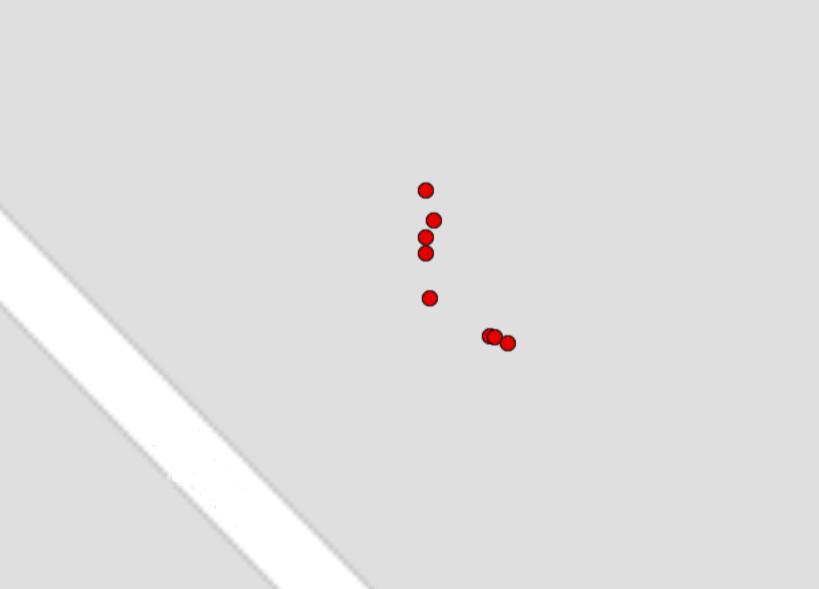
\includegraphics[width=3in]{img/mapka_punktygps.png}
\captionsetup{justification=centering}
\captionof{figure}{Wizualizacja współrzędnych nieporuszającego się odbiornika na mapie. [Opracowanie własne]}
\label{fig:mapka_punktygps}
}
\end{table}%

Zignorowanie powyższego zjawiska, mogłoby doprowadzić do bardzo niekorzystnej sytuacji. Gdyby osoba tworząca trasę zatrzymała się w trakcie treningu, na przykład w~celu odpoczynku lub zawiązania buta, zapisany przebieg treningu zawierałby skupisko fałszywych punktów. W celu wyeliminowania tego zagrożenia, podczas tworzenia trasy brane są pod uwagę tylko te punkty, które są oddalone od poprzedniego o więcej niż 15 metrów. Dzięki temu chwilowe zatrzymanie się podczas treningu, nie powoduje powstania przekłamań w~generowanej trasie.
\subsection{Zapobieganie oszustwom}\label{chap:zapobieganie-oszustwom}
Opieranie rywalizacji biegowej jednie na danych pobieranych z systemów nawigacji satelitarnej, sprawia że jej uczciwość może być zaburzona w stosunkowo łatwy sposób. Nic nie stoi na przeszkodzie, aby do pokonania trasy użyć chociażby roweru. Możliwe jest także manualne wprowadzanie danych lokalizacyjnych do urządzenia \cite{fakegps}, co pozwoli uzyskać dowolnie dobry wynik bez podejmowania jakiejkolwiek aktywności fizycznej. Zagrożenia tego można uniknąć na dwa sposoby:
\begin{itemize}
\item{\textbf{Porównywanie osiąganych przez użytkowników rezultatów z wynikami najlepszych na świecie biegaczy}} - Zapisanie w aplikacji zbioru światowych rekordów biegowych na konkretnych dystansach i porównywanie ich do wyników uzyskiwanych przez użytkowników jest pierwszym ze sposobów na zapobieganie oszustwom. Rezultaty znacząco lepsze od tych, które zostały osiągnięte na atestowanych zawodach z całą pewnością mogą zostać uznane jako osiągnięte nieuczciwie. Choć rozwiązanie to zapobiegnie zapisywaniu w rankingu czasów trasy, które są wręcz niemożliwe do osiągnięcia, nie sprawdzi się w przypadkach gdy sfałszowany wynik mieści się w granicach zdrowego rozsądku.
\item{\textbf{Skorzystanie z czujników dostępnych w urządzeniu}} - Akcelerometr oraz żyroskop są jednymi z wielu czujników umieszczanych w produkowanych obecnie telefonach komórkowych. Ich zadaniem jest mierzenie przyspieszenia liniowego oraz położenia kątowego \cite{czujniki}. Umożliwiają zatem pozyskanie informacji o ruchach jakim poddane jest urządzenie w trakcie trwania treningu. Opracowanie odpowiedniego algorytmu oraz skorzystanie z sieci neuronowych pozwoliłyby stwierdzić, czy dane pobrane z czujników w~czasie odbywania treningu, zgadzają się z tymi, które generowane są w czasie biegu i na tej podstawie dokonać akceptacji lub unieważnienia próby użytkownika. W~przeciwieństwie do poprzedniego podejścia, bieżące rozwiązanie okazałoby się skuteczne także w~przypadkach, w których dane lokalizacyjne zostały wprowadzone do urządzenia manualnie oraz gdy osiągnięty na trasie rezultat nie jest lepszy niż ogólnoświatowe rekordy. Rozwiązanie tego problemu obejmuje zagadnienia z dziedziny sztucznej inteligencji i wykracza poza zakres niniejszej pracy, dlatego też nie zostało zaimplementowane w tworzonej aplikacji.
\end{itemize}

\section{Istniejące rozwiązania w dziedzinie aplikacji treningowych}\label{chap:istniejace}
Na rynku aplikacji znajduje się wiele aplikacji, których przeznaczeniem jest wspieranie treningów biegowych. Pozwalają one użytkownikom na dogłębną analizę aktywności sportowych oraz śledzenie treningów zarówno swoich jak i udostępnianych przez innych biegaczy. Funkcjonalności te są bardzo powszechne. Nie udało się znaleźć aplikacji treningowej, która w pełni oferuje funkcjonalność zawartą w rozwiązaniu, które budowane jest w ramach niniejszej pracy, dlatego do niniejszego przeglądu wybrano trzy przykłady aplikacji, których zakres działania jest jak najbardziej do niej zbliżony, a jednocześnie cieszących się wysoką oceną oraz popularnością w sklepie z aplikacjami Google Play \cite{googleplay}. 
\subsection{Endomondo}
Jedną z najwcześniej wydanych (pierwsze wersja została udostępniona w listopadzie 2007 roku), a zarówno najbardziej popularnych na świecie aplikacji jest Endomondo \cite{endomondo}.  Pozwala na śledzenie aktywności w ponad 60 dyscyplinach sportowych, włączając w~to bieganie. W aplikacji rozwinięto aspekt społecznościowy - znajomi mają możliwość wzajemnego przeglądania historii swoich treningów. Ich statystyki mogą być także udostępniane na mediach społecznościowych. Ponadto istnieje możliwość tworzenia własnych tras, które inni biegacze mogą następnie przeglądać w formie listy i używać do własnych treningów. Niestety możliwe jest zobaczenie tylko całego zbioru tras, znajdujących się w pewnej nieznanej odległości od użytkownika. Stanowi to problem, ponieważ nie mogąc określić dokładnie obszaru wyszukiwania, biegacze nie są pewni, czy zobaczyli już wszystkie trasy, które mogłyby ich potencjalnie zainteresować czy może istnieje ich więcej, ale znajdują się poza nieznanym obszarem wyszukiwania. Producent nie udostępnił także możliwości filtrowania wyników wyszukiwania ze względu na długość trasy, twardość nawierzchni czy poziom terenu. Podczas tworzenia trasy zapisywana jest co prawda jej całkowita długość, jednak służy ona tylko poinformowaniu użytkownika, a nie wyszukiwaniu. Aplikacja nie pozwala także na jakiekolwiek porównywanie wyników, które biegacze osiągają na trasie.
\subsection{Strava}
Strava \cite{strava} jest aplikacją, która w momencie pisania niniejszej pracy wspiera treningi w~24 dyscyplinach sportowych. Oprócz podstawowej funkcjonalności aplikacji treningowych, oferuje także analizę treningów na podstawie rozmaitych statystyk i~wykresów. Aplikacja umożliwia także funkcję tworzenia i zapisywania tras. Oprócz samego jej przebiegu, zapisywana jest także jej długość oraz poziom terenu. Niestety, tak jak w przypadku aplikacji Endomondo, producent nie umożliwił filtrowania tras według żadnej z tych cech. Podczas przeglądania tras, ukazują się one na interaktywnej mapie, którą można przesuwać. Nie występuje tutaj zatem znany z Endomondo problem niemożności określenia obszaru, w którym wyszukiwane są trasy. Rozszerzenie obszaru poszukiwania ogranicza się do przesunięcia mapy na ekranie urządzenia. Zapisywanie czasów użytkowników którzy ukończyli trasę na serwerze, pozwala użytkownikom na wyświetlenie rankingu trasy i porównanie swojej dyspozycji do innych biegaczy. Funkcjonalność ta daje poczucie pewnego rodzaju rywalizacji, jednak sprawdzenie uzyskanego wyniku możliwe jest dopiero po ukończeniu treningu, użytkownik nie otrzymuje na ten temat informacji w czasie jego trwania.
\subsection{MapMyRun}
Przeznaczeniem aplikacji MapMyRun \cite{mapmyrun} jest przede wszystkim śledzenie aktywności związanych ze spacerowaniem i bieganiem. W tym przykładzie użytkownicy także mają możliwość przeglądania i analizowania swoich poprzednich treningów. Usprawnieniem jest fakt, iż trasy można filtrować na podstawie ich długości. Zabrakło niestety filtra poziomu terenu, mimo że informacja ta jest zapisywana podczas tworzenia trasy. Podczas wyszukiwania tras pojawia się problem znany z aplikacji Endomondo - prezentowane trasy należą do obszaru, którego granice oddalone są od użytkownika o~nieznaną odległość, przez co biegacze nie są pewni czy zostały im wyświetlone wszystkie godne uwagi trasy czy może część z nich znajduje się poza obszarem poszukiwań. Element rywalizacji jest zorganizowany podobnie jak w aplikacji Strava - wyniki osiągane przez użytkowników są zapisywane na serwerze, dzięki czemu mają oni możliwość sprawdzenia swojej dyspozycji po zakończonym treningu.
\chapter{Tworzenie i charakterystyka tras}\label{chap:charakterystyka-tras}
Tworzenie trasy polega na zapisaniu w systemie pozycji, ustalonych przy użyciu nawigacji satelitarnej, na których użytkownik znajdował się w trakcie treningu tak jak zostało to pokazane na rysunku przedstawiającym fragment utworzonej trasy \ref{image:mapka_fragment_trasy}, na którym linią ciągłą zaznaczono rzeczywistą trasę pokonaną przez biegacza, a kropkami reprezentację trasy zapisaną w systemie. Zapamiętywane są tylko te punkty, które znajdują się w odległości nie mniejszej niż 10 metrów od swojego poprzednika. Zaproponowana minimalna odległość pomiędzy punktami, pozwoli na osiągnięcie dostatecznie dokładnego przebiegu trasy, przy jednoczesnym zapobiegnięciu wystąpienia problemu, opisanego w rozdziale \ref{chap:wahania-pozycji}.

\begin{figure}[h]\label{fig:miary}
\begin{center}
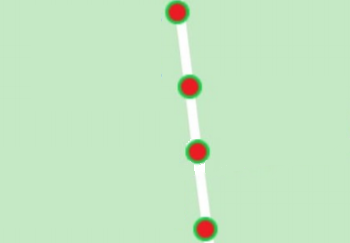
\includegraphics{img/mapka_fragment_trasy.png}
\caption{Fragment utworzonej trasy. [Opracowanie własne]}\label{image:mapka_fragment_trasy}
\end{center}
\end{figure}

Zawody biegowe w których biegacze biorą udział, różnią się trasami, na jakich są przeprowadzane. Ich dystans może wynosić od kilku do kilkudziesięciu kilometrów. Zawody odbywające się w mieście zwykle odbywają się na płaskiej nawierzchni asfaltowej, podczas gdy biegi organizowane w górach wymagają często od zawodników podbiegania pod jakiś szczyt górski lub zbiegania z niego. Nie inaczej jest z przygotowaniem do konkretnych zawodów. Chcąc jak najefektywniej przygotować się do startu, biegacz powinien trenować w warunkach zbliżonych do tych, które może spotkać na zawodach. Z tego względu aplikacja tworzona w ramach niniejszej pracy umożliwia użytkownikom wyszukiwanie tras treningowych, które spełnią ich preferencje. Niniejszy rozdział jest realizacją części pierwszego celu przedstawionego w rozdziale \ref{chap:cele-pracy}. Omówiono w nim cechy, które mogą zostać przypisane do trasy, sposób ich wyznaczenia na podstawie danych lokalizacyjnych oraz kryteria wyszukiwania używane podczas przeglądania tras. 
\section{Możliwe cechy trasy}\label{chap:opis-cech}
Do każdej trasy mogą zostać przypisane 3 cechy.
\begin{itemize}
\item{\textbf{Dystans}} - określa jak długa jest trasa. Wartość wyrażona jest w kilometrach.
\item{\textbf{Poziom terenu}} - Reprezentuje zmianę wysokości nad poziomem morza pomiędzy początkiem a końcem trasy. Wartości które może przyjąć ta cecha to:
\begin{itemize}
\item{Wyrównany} - gdy wysokość nad poziomem morze nie zmienia się lub zmienia się nieznacznie,
\item{Rosnący} - gdy wysokość nad poziomem morza wzrasta,
\item{Malejący} - gdy wysokość nad poziomem morza maleje.
\end{itemize}
\item{\textbf{Twardość nawierzchni}} - Wyraża jaka część całej trasy przebiega przez nawierzchnię utwardzoną (na przykład asfalt lub kostka brukowa) w stosunku do nawierzchni nieutwardzonej (na przykład piasek lub trawa). Wartość wyrażona jest w procentach. Przykładowo wartość 60\% dla trasy o dystansie 10 kilometrów oznacza, że 6 kilometrów prowadzi przez nawierzchnię utwardzoną, a 4 kilometry przez nieutwardzoną.
\end{itemize}
\section{Przypisanie cech do trasy}
Długość trasy przypisywana jest bezpośrednio po ukończeniu treningu. Jej wyznaczenie polega na zsumowaniu odległości pomiędzy wszystkimi następującymi po sobie punktami przy użyciu wzorów \ref{eq:haversine1},  \ref{eq:haversine2} i \ref{eq:haversine3}.

Określenie poziomu terenu odbywa się poprzez obliczenie różnicy wysokości nad poziomem morza pomiędzy punktem rozpoczynającym oraz kończącym trasę i przypisanie odpowiednio poziomu:
\begin{itemize}
\item{\textbf{wyrównanego}} - gdy różnica nie przekracza 10\%,
\item{\textbf{rosnącego}} - gdy wysokość punktu końcowego jest większa od wysokości punktu początkowego o więcej niż 10\%,
\item{\textbf{malejącego}} - gdy wysokość punktu początkowego jest większa od wysokości punktu końcowego o więcej niż 10\%.
\end {itemize}
Należy mieć na uwadze, że w przypadku wystąpienia problemu opisanego w rozdziale \ref{chap:problem-poziom-terenu}, cecha ta będzie musiała zostać ustalona przez użytkownika.

W celu umożliwienia automatycznego przypisania rodzaju nawierzchni, posłużono się serwisem OpenStreetMap \cite{osm}. Narzędzie to pozwala scharakteryzować podłoże ustalonego przez klienta obszaru. Musi on być zdefiniowany w formie prostokąta, a odbywa się to poprzez dostarczenie serwisowi współrzędnych geograficznych jego lewej dolnej oraz prawej górnej krawędzi. Zdefiniowane przykładowego obszaru zostało pokazane na rysunku \ref{image:mapka_obszar}. Kropkami oznaczono podane współrzędne geograficzne, natomiast linia ciągła definiuje obszar, który zostanie poddany analizie. W odpowiedzi klient otrzymuje charakterystykę wszystkich dróg, które znalazły się w zdefiniowanym obszarze \cite{osm-docs-wiki}. Rodzaj nawierzchni nie jest zwracany w formie „utwardzona” bądź „nieutwardzona”, lecz w formie sprecyzowanej, na przykład „asfalt” lub „trawa”, dlatego pierwszym krokiem którego trzeba się podjąć po otrzymaniu odpowiedzi, jest przyporządkowanie etykiety  „utwardzona” bądź „nieutwardzona” dla każdego z otrzymanych obiektów. Przyporządkowanie wszystkich możliwych do otrzymania rodzajów nawierzchni zostało pokazane w tabeli \ref{table:rodzaje-nawierzchni} \cite{osm-surface}.

\begin{figure}[h]\label{fig:miary}
\begin{center}
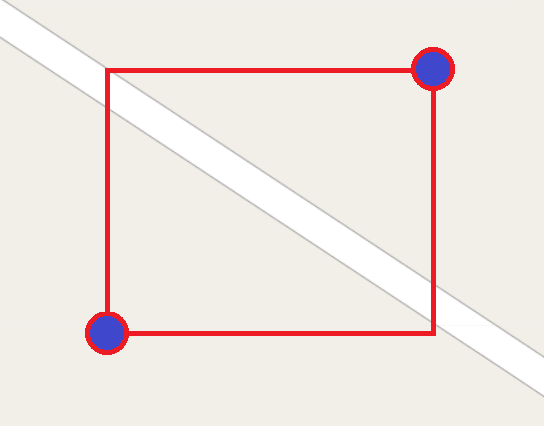
\includegraphics[width=2in]{img/mapka_obszar.png}
\caption{Obszar poddany analizie [Opracowanie własne]}\label{image:mapka_obszar}
\end{center}
\end{figure}

\begin{table}[thb]
\caption{Przyporządkowanie konkretnego rodzaju nawierzchni do jej reprezentacji w tworzonym systemie \cite{osm-surface}}.\label{table:rodzaje-nawierzchni}
\centering\renewcommand\cellalign{lc}
\setcellgapes{3pt}\makegapedcells
\begin{tabular}{|c|c|} \hline
\textbf{Nawierzchnia utwardzona} & \textbf{Nawierzchnia nieutwardzona} \\ \hline
\makecell{paved, asphalt, concrete,\\concrete:lanes, concrete:plates,\\paving\textunderscore stones, sett,\\unhewn\textunderscore cobblestone,\\cobblestone, metal, wood,\\metal\textunderscore grid } & \makecell{ unpaved, compacted, fine\textunderscore gravel,\\gravel, pebblestone, dirt,\\earth, grass, grass\textunderscore paver,\\ground, mud, sand, woodchips,\\snow, ice, salt, clay, tartan,\\artifical\textunderscore turf, decoturf, carpet} \\ \hline
\end{tabular}
\end{table}

Tworzone przez użytkowników trasy zapisywane są w formie punktów, dlatego przed skorzystaniem z serwisu OpenStreetMap, należy zdefiniować wspomniany prostokątny obszar poszukiwań. Korzystając ze wzoru \cite{eq:haversine_generowanie_punktu} wyznaczane są więc 2 nowe punkty: oddalony o 10 metrów i 225 stopni względem północy oraz oddalony o 10 metrów i 45 stopni względem północy. Po ustaleniu rodzaju nawierzchni dla każdego z punktów trasy, możliwe jest wyliczenie wartości procentowej, a tym samym określenie cechy według wzoru:
\begin{equation}\label{eq:haversine1}
{Twardość\hspace{0.15cm} nawierzchni} = \frac{u}{u + n} \cdot 100,
\end{equation}
gdzie \(u\) oznacza liczbę obiektów z etykietą  „utwardzona”, \(n\) liczbę obiektów z etykietą  „nieutwardzona”.
Z uwagi na czytelność wynik zaokrąglany jest do liczby całkowitej.
Należy mieć na uwadze, że OpenStreetMap jest projektem tworzonym przez społeczność i dla pewnych dróg rodzaj nawierzchni mógł być przypisany błędnie bądź nie przypisany wcale. Wartość określonej cechy powinna być zatem traktowana w formie propozycji, którą użytkownik tworzący trasę może poprawić wedle własnego uznania.

\section{Kryteria wyszukiwania tras}
Kryteria wyszukiwania są ściśle powiązane z cechami opisanymi w rozdziale \ref{chap:opis-cech}. Dokonano jedynie kilku usprawnień mających na celu wygodę użytkownika.
\begin{itemize}
\item{Kryterium \textbf{długości trasy} przyjmuje wartości „od” oraz „do”. Oznacza to, że lista wynikowa zawiera trasy nie krótsze niż pierwsza z nich, a jednocześnie nie dłuższe niż druga z nich. Największa wartość, którą można określić wynosi 20 kilometrów.  Po jej przekroczeniu, przy wyszukiwaniu pod uwagę brane są trasy o nieograniczonej maksymalnej długości,}
\item{Przy filtrowaniu ze względu na \textbf{poziom terenu} oprócz konkretnych wartości cechy możliwe jest także wybranie opcji „każdy”. Oznacza to, że trasy nie będą filtrowane według tej cechy.}
\item{\textbf{Twardość nawierzchni} podobnie jak w przypadku długości trasy określana jest jako zakres  „od, do”. Wartość maksymalna wynosi 100\%.}
\end{itemize}
Oprócz tego użytkownik musi określić maksymalny promień wyszukiwania względem jego obecnej lokalizacji. Dzięki temu jest on świadomy, że zostały mu pokazane wszystkie trasy z interesującego go obszaru. Nie bez znaczenia jest także fakt, że zapobiegnie to pobieraniu z bazy danych wszystkich istniejących tras, co miałoby znaczący wpływ na wykorzystanie łącza oraz wydajność zarówno aplikacji serwerowej jak i aplikacji mobilnej.
\bibliographystyle{plain}
\bibliography{sample.bib}
\listoffigures
\listoftables
\end{document}